% !TEX root = tnnls_relation_gait.tex

\ifx\allfiles\undefined
    % !TEX root = tnnls_relation_gait.tex

%% bare_jrnl.tex
%% V1.4b
%% 2015/08/26
%% by Michael Shell
%% see http://www.michaelshell.org/
%% for current contact information.
%%
%% This is a skeleton file demonstrating the use of IEEEtran.cls
%% (requires IEEEtran.cls version 1.8b or later) with an IEEE
%% journal paper.
%%
%% Support sites:
%% http://www.michaelshell.org/tex/ieeetran/
%% http://www.ctan.org/pkg/ieeetran
%% and
%% http://www.ieee.org/

%%*************************************************************************
%% Legal Notice:
%% This code is offered as-is without any warranty either expressed or
%% implied; without even the implied warranty of MERCHANTABILITY or
%% FITNESS FOR A PARTICULAR PURPOSE!
%% User assumes all risk.
%% In no event shall the IEEE or any contributor to this code be liable for
%% any damages or losses, including, but not limited to, incidental,
%% consequential, or any other damages, resulting from the use or misuse
%% of any information contained here.
%%
%% All comments are the opinions of their respective authors and are not
%% necessarily endorsed by the IEEE.
%%
%% This work is distributed under the LaTeX Project Public License (LPPL)
%% ( http://www.latex-project.org/ ) version 1.3, and may be freely used,
%% distributed and modified. A copy of the LPPL, version 1.3, is included
%% in the base LaTeX documentation of all distributions of LaTeX released
%% 2003/12/01 or later.
%% Retain all contribution notices and credits.
%% ** Modified files should be clearly indicated as such, including  **
%% ** renaming them and changing author support contact information. **
%%*************************************************************************


% *** Authors should verify (and, if needed, correct) their LaTeX system  ***
% *** with the testflow diagnostic prior to trusting their LaTeX platform ***
% *** with production work. The IEEE's font choices and paper sizes can   ***
% *** trigger bugs that do not appear when using other class files.       ***                          ***
% The testflow support page is at:
% http://www.michaelshell.org/tex/testflow/

\documentclass[journal]{IEEEtran}
%
% If IEEEtran.cls has not been installed into the LaTeX system files,
% manually specify the path to it like:
% \documentclass[journal]{../sty/IEEEtran}

% Some very useful LaTeX packages include:
% (uncomment the ones you want to load)

% *** MISC UTILITY PACKAGES ***
%
%\usepackage{ifpdf}
% Heiko Oberdiek's ifpdf.sty is very useful if you need conditional
% compilation based on whether the output is pdf or dvi.
% usage:
% \ifpdf
%   % pdf code
% \else
%   % dvi code
% \fi
% The latest version of ifpdf.sty can be obtained from:
% http://www.ctan.org/pkg/ifpdf
% Also, note that IEEEtran.cls V1.7 and later provides a builtin
% \ifCLASSINFOpdf conditional that works the same way.
% When switching from latex to pdflatex and vice-versa, the compiler may
% have to be run twice to clear warning/error messages.

% *** CITATION PACKAGES ***

\usepackage{tabularx}
\usepackage{longtable}
\usepackage{threeparttable}
\usepackage{cite}

% cite.sty was written by Donald Arseneau
% V1.6 and later of IEEEtran pre-defines the format of the cite.sty package
% \cite{} output to follow that of the IEEE. Loading the cite package will
% result in citation numbers being automatically sorted and properly
% "compressed/ranged". e.g., [1], [9], [2], [7], [5], [6] without using
% cite.sty will become [1], [2], [5]--[7], [9] using cite.sty. cite.sty's
% \cite will automatically add leading space, if needed. Use cite.sty's
% noadjust option (cite.sty V3.8 and later) if you want to turn this off
% such as if a citation ever needs to be enclosed in parenthesis.
% cite.sty is already installed on most LaTeX systems. Be sure and use
% version 5.0 (2009-03-20) and later if using hyperref.sty.
% The latest version can be obtained at:
% http://www.ctan.org/pkg/cite
% The documentation is contained in the cite.sty file itself.

% *** GRAPHICS RELATED PACKAGES ***
%
\usepackage[pdftex]{graphicx}
\usepackage{rotating}
\ifCLASSINFOpdf
  % \usepackage[pdftex]{graphicx}
  % declare the path(s) where your graphic files are
  % \graphicspath{{../pdf/}{../jpeg/}}
  % and their extensions so you won't have to specify these with
  % every instance of \includegraphics
  % \DeclareGraphicsExtensions{.pdf,.jpeg,.png}
\else
  % or other class option (dvipsone, dvipdf, if not using dvips). graphicx
  % will default to the driver specified in the system graphics.cfg if no
  % driver is specified.
  % \usepackage[dvips]{graphicx}
  % declare the path(s) where your graphic files are
  % \graphicspath{{../eps/}}
  % and their extensions so you won't have to specify these with
  % every instance of \includegraphics
  % \DeclareGraphicsExtensions{.eps}
\fi
% graphicx was written by David Carlisle and Sebastian Rahtz. It is
% required if you want graphics, photos, etc. graphicx.sty is already
% installed on most LaTeX systems. The latest version and documentation
% can be obtained at:
% http://www.ctan.org/pkg/graphicx
% Another good source of documentation is "Using Imported Graphics in
% LaTeX2e" by Keith Reckdahl which can be found at:
% http://www.ctan.org/pkg/epslatex
%
% latex, and pdflatex in dvi mode, support graphics in encapsulated
% postscript (.eps) format. pdflatex in pdf mode supports graphics
% in .pdf, .jpeg, .png and .mps (metapost) formats. Users should ensure
% that all non-photo figures use a vector format (.eps, .pdf, .mps) and
% not a bitmapped formats (.jpeg, .png). The IEEE frowns on bitmapped formats
% which can result in "jaggedy"/blurry rendering of lines and letters as
% well as large increases in file sizes.
%
% You can find documentation about the pdfTeX application at:
% http://www.tug.org/applications/pdftex

% *** MATH PACKAGES ***
%
\usepackage{amsmath}
% A popular package from the American Mathematical Society that provides
% many useful and powerful commands for dealing with mathematics.
%
% Note that the amsmath package sets \interdisplaylinepenalty to 10000
% thus preventing page breaks from occurring within multiline equations. Use:
%\interdisplaylinepenalty=2500
% after loading amsmath to restore such page breaks as IEEEtran.cls normally
% does. amsmath.sty is already installed on most LaTeX systems. The latest
% version and documentation can be obtained at:
% http://www.ctan.org/pkg/amsmath

% *** SPECIALIZED LIST PACKAGES ***
%
\usepackage{algorithmic}
% algorithmic.sty was written by Peter Williams and Rogerio Brito.
% This package provides an algorithmic environment fo describing algorithms.
% You can use the algorithmic environment in-text or within a figure
% environment to provide for a floating algorithm. Do NOT use the algorithm
% floating environment provided by algorithm.sty (by the same authors) or
% algorithm2e.sty (by Christophe Fiorio) as the IEEE does not use dedicated
% algorithm float types and packages that provide these will not provide
% correct IEEE style captions. The latest version and documentation of
% algorithmic.sty can be obtained at:
% http://www.ctan.org/pkg/algorithms
% Also of interest may be the (relatively newer and more customizable)
% algorithmicx.sty package by Szasz Janos:
% http://www.ctan.org/pkg/algorithmicx

% *** ALIGNMENT PACKAGES ***
%
\usepackage{array}
% Frank Mittelbach's and David Carlisle's array.sty patches and improves
% the standard LaTeX2e array and tabular environments to provide better
% appearance and additional user controls. As the default LaTeX2e table
% generation code is lacking to the point of almost being broken with
% respect to the quality of the end results, all users are strongly
% advised to use an enhanced (at the very least that provided by array.sty)
% set of table tools. array.sty is already installed on most systems. The
% latest version and documentation can be obtained at:
% http://www.ctan.org/pkg/array

% IEEEtran contains the IEEEeqnarray family of commands that can be used to
% generate multiline equations as well as matrices, tables, etc., of high
% quality.

% *** SUBFIGURE PACKAGES ***
\usepackage[caption=false,font=footnotesize]{subfig}
%\ifCLASSOPTIONcompsoc
%  \usepackage[caption=false,font=normalsize,labelfont=sf,textfont=sf]{subfig}
%\else
%  \usepackage[caption=false,font=footnotesize]{subfig}
%\fi
% subfig.sty, written by Steven Douglas Cochran, is the modern replacement
% for subfigure.sty, the latter of which is no longer maintained and is
% incompatible with some LaTeX packages including fixltx2e. However,
% subfig.sty requires and automatically loads Axel Sommerfeldt's caption.sty
% which will override IEEEtran.cls' handling of captions and this will result
% in non-IEEE style figure/table captions. To prevent this problem, be sure
% and invoke subfig.sty's "caption=false" package option (available since
% subfig.sty version 1.3, 2005/06/28) as this is will preserve IEEEtran.cls
% handling of captions.
% Note that the Computer Society format requires a larger sans serif font
% than the serif footnote size font used in traditional IEEE formatting
% and thus the need to invoke different subfig.sty package options depending
% on whether compsoc mode has been enabled.
%
% The latest version and documentation of subfig.sty can be obtained at:
% http://www.ctan.org/pkg/subfig

% *** FLOAT PACKAGES ***
%
%\usepackage{fixltx2e}
% fixltx2e, the successor to the earlier fix2col.sty, was written by
% Frank Mittelbach and David Carlisle. This package corrects a few problems
% in the LaTeX2e kernel, the most notable of which is that in current
% LaTeX2e releases, the ordering of single and double column floats is not
% guaranteed to be preserved. Thus, an unpatched LaTeX2e can allow a
% single column figure to be placed prior to an earlier double column
% figure.
% Be aware that LaTeX2e kernels dated 2015 and later have fixltx2e.sty's
% corrections already built into the system in which case a warning will
% be issued if an attempt is made to load fixltx2e.sty as it is no longer
% needed.
% The latest version and documentation can be found at:
% http://www.ctan.org/pkg/fixltx2e

%\usepackage{stfloats}
% stfloats.sty was written by Sigitas Tolusis. This package gives LaTeX2e
% the ability to do double column floats at the bottom of the page as well
% as the top. (e.g., "\begin{figure*}[!b]" is not normally possible in
% LaTeX2e). It also provides a command:
%\fnbelowfloat
% to enable the placement of footnotes below bottom floats (the standard
% LaTeX2e kernel puts them above bottom floats). This is an invasive package
% which rewrites many portions of the LaTeX2e float routines. It may not work
% with other packages that modify the LaTeX2e float routines. The latest
% version and documentation can be obtained at:
% http://www.ctan.org/pkg/stfloats
% Do not use the stfloats baselinefloat ability as the IEEE does not allow
% \baselineskip to stretch. Authors submitting work to the IEEE should note
% that the IEEE rarely uses double column equations and that authors should try
% to avoid such use. Do not be tempted to use the cuted.sty or midfloat.sty
% packages (also by Sigitas Tolusis) as the IEEE does not format its papers in
% such ways.
% Do not attempt to use stfloats with fixltx2e as they are incompatible.
% Instead, use Morten Hogholm'a dblfloatfix which combines the features
% of both fixltx2e and stfloats:
%
% \usepackage{dblfloatfix}
% The latest version can be found at:
% http://www.ctan.org/pkg/dblfloatfix

%\ifCLASSOPTIONcaptionsoff
%  \usepackage[nomarkers]{endfloat}
% \let\MYoriglatexcaption\caption
% \renewcommand{\caption}[2][\relax]{\MYoriglatexcaption[#2]{#2}}
%\fi
% endfloat.sty was written by James Darrell McCauley, Jeff Goldberg and
% Axel Sommerfeldt. This package may be useful when used in conjunction with
% IEEEtran.cls'  captionsoff option. Some IEEE journals/societies require that
% submissions have lists of figures/tables at the end of the paper and that
% figures/tables without any captions are placed on a page by themselves at
% the end of the document. If needed, the draftcls IEEEtran class option or
% \CLASSINPUTbaselinestretch interface can be used to increase the line
% spacing as well. Be sure and use the nomarkers option of endfloat to
% prevent endfloat from "marking" where the figures would have been placed
% in the text. The two hack lines of code above are a slight modification of
% that suggested by in the endfloat docs (section 8.4.1) to ensure that
% the full captions always appear in the list of figures/tables - even if
% the user used the short optional argument of \caption[]{}.
% IEEE papers do not typically make use of \caption[]'s optional argument,
% so this should not be an issue. A similar trick can be used to disable
% captions of packages such as subfig.sty that lack options to turn off
% the subcaptions:
% For subfig.sty:
% \let\MYorigsubfloat\subfloat
% \renewcommand{\subfloat}[2][\relax]{\MYorigsubfloat[]{#2}}
% However, the above trick will not work if both optional arguments of
% the \subfloat command are used. Furthermore, there needs to be a
% description of each subfigure *somewhere* and endfloat does not add
% subfigure captions to its list of figures. Thus, the best approach is to
% avoid the use of subfigure captions (many IEEE journals avoid them anyway)
% and instead reference/explain all the subfigures within the main caption.
% The latest version of endfloat.sty and its documentation can obtained at:
% http://www.ctan.org/pkg/endfloat
%
% The IEEEtran \ifCLASSOPTIONcaptionsoff conditional can also be used
% later in the document, say, to conditionally put the References on a
% page by themselves.

% *** PDF, URL AND HYPERLINK PACKAGES ***
%
\usepackage{url}
% url.sty was written by Donald Arseneau. It provides better support for
% handling and breaking URLs. url.sty is already installed on most LaTeX
% systems. The latest version and documentation can be obtained at:
% http://www.ctan.org/pkg/url
% Basically, \url{my_url_here}.

% *** Do not adjust lengths that control margins, column widths, etc. ***
% *** Do not use packages that alter fonts (such as pslatex).         ***
% There should be no need to do such things with IEEEtran.cls V1.6 and later.
% (Unless specifically asked to do so by the journal or conference you plan
% to submit to, of course. )

% correct bad hyphenation here
% \hyphenation{op-tical net-works semi-conduc-tor}
\usepackage{enumerate}
\usepackage{multirow}
\usepackage{color}
\usepackage{threeparttable}
\usepackage{booktabs}
\newcommand{\minus}{\scalebox{0.75}[1.0]{$-$}}
\newcommand{\bftab}[1]{{\fontseries{b}\selectfont#1}}
\newcommand{\tabincell}[2]{\begin{tabular}{@{}#1@{}}#2\end{tabular}}
\newcommand{\etal}{\textit{et al}.}
\newcommand{\ie}{\textit{i.e.}}
\newcommand{\eg}{\textit{e.g.}}
\newcommand{\wrt}{\textit{w.r.t.}}
\newcommand{\vs}{\textit{vs.}}


\begin{document}
%
% paper title
% Titles are generally capitalized except for words such as a, an, and, as,
% at, but, by, for, in, nor, of, on, or, the, to and up, which are usually
% not capitalized unless they are the first or last word of the title.
% Linebreaks \\ can be used within to get better formatting as desired.
% Do not put math or special symbols in the title.
%\title{The Application and Research of Multi-modal Data in Auxiliary Diagnosis of Depression: A Survey
%}
\title{ Auxiliary Diagnosis of Depression Based on Multi-modal Data: A Survey
}
%%
%%
%% author names and IEEE memberships
%% note positions of commas and nonbreaking spaces ( ~ ) LaTeX will not break
%% a structure at a ~ so this keeps an author's name from being broken across
%% two lines.
%% use \thanks{} to gain access to the first footnote area
%% a separate \thanks must be used for each paragraph as LaTeX2e's \thanks
%% was not built to handle multiple paragraphs
%%
%
%\author{Saihui~Hou,
%	Xu~Liu,
%	Chunshui~Cao,
%	and~Yongzhen~Huang$^*$% <-this % stops a space
%	\thanks{$^*$ indicates the corresponding author.}% <-this % stops a space
%    \thanks{Saihui Hou and Yongzhen Huang is with School of Artificial Intelligence, Beijing Normal University, Beijing 100875, China. (Email: housaihui@bnu.edu.cn, huangyongzhen@bnu.edu.cn)}
%	\thanks{Xu Liu and Chunshui Cao are with Watrix Technology Limited Co. Ltd, Beijing 100088, China. (Email: xu.liu@watrix.ai, chunshuicao@watrix.ai)}
%    \thanks{This work is partially supported by the Fundamental Research Funds for the Central Universities.}
%    % \thanks{E-mail: housaihui@bnu.edu.cn, xu.liu@watrix.ai, chunshuicao@watrix.ai, huangyongzhen@bnu.edu.cn}
%	% \thanks{Manuscript received April 19, 2005; revised August 26, 2015.}
%}
%
%% note the % following the last \IEEEmembership and also \thanks -
%% these prevent an unwanted space from occurring between the last author name
%% and the end of the author line. i.e., if you had this:
%%
%% \author{....lastname \thanks{...} \thanks{...} }
%%                     ^------------^------------^----Do not want these spaces!
%%
%% a space would be appended to the last name and could cause every name on that
%% line to be shifted left slightly. This is one of those "LaTeX things". For
%% instance, "\textbf{A} \textbf{B}" will typeset as "A B" not "AB". To get
%% "AB" then you have to do: "\textbf{A}\textbf{B}"
%% \thanks is no different in this regard, so shield the last } of each \thanks
%% that ends a line with a % and do not let a space in before the next \thanks.
%% Spaces after \IEEEmembership other than the last one are OK (and needed) as
%% you are supposed to have spaces between the names. For what it is worth,
%% this is a minor point as most people would not even notice if the said evil
%% space somehow managed to creep in.
%
%% The paper headers
%\markboth{IEEE Transactions on Neural Networks and Learning Systems}%
%{Saihui Hou \MakeLowercase{\textit{et al.}}: GQAN: Towards the Interpretability of Silhouette-based Gait Recognition}
%% The only time the second header will appear is for the odd numbered pages
%% after the title page when using the twoside option.
%%
%% *** Note that you probably will NOT want to include the author's ***
%% *** name in the headers of peer review papers.                   ***
%% You can use \ifCLASSOPTIONpeerreview for conditional compilation here if
%% you desire.
%
%% If you want to put a publisher's ID mark on the page you can do it like
%% this:
%%\IEEEpubid{0000--0000/00\$00.00~\copyright~2015 IEEE}
%% Remember, if you use this you must call \IEEEpubidadjcol in the second
%% column for its text to clear the IEEEpubid mark.
%
%% use for special paper notices
%%\IEEEspecialpapernotice{(Invited Paper)}
%
%% make the title area
\maketitle

\fi
%\section{Depression Recognition}
%\section{Depression recognition method based on audiovisual}
\subsection{Speech}

Speech is a non-invasive signal that is low-cost and easily accessible.
The study of speech-based depression recognition began with the examination of clinical aspects of depressed individuals' speech.
Clinical observations have revealed that there are phonetic differences in speech between healthy and depressed populations.
These differences can be seen in the fact that depressed people typically speak more smoothly and monotonously, whereas healthy people speak more rhythmically, with less pauses and fewer times than depressed people\cite{pampouchidou2017facial,montgomery1979new}.
Furthermore, the researchers  designed characteristics based on the variations between the two groups. These characteristics are objective in nature and are able to discriminate between populations that are healthy and those that are depressed.
But with the rapid advancement of deep learning techniques in recent years, speech-based depression recognition has transitioned from hand-crafted acoustic features to a deep learning-based framework.
%
%Previous work for depression
%analysis can be broadly categorized into handcrafted feature based
%methods and deep learning feature based methods according to
%their adopted frameworks.


\subsubsection{Speech depression recognition based on traditional machine learning}

So far, automatic speech-based depression analysis has primarily relied on classic machine learning methods supplemented with hand-crafted feature, as shown in Fig.\ref{Speech01}.
In terms of hand-crafted feature engineering, the major work is to learn acoustic features related to depression and experiment with feature sets to improve performance.
Researchers have also employed classic machine learning algorithms, such as support vector machines, as classifiers for depression diagnosis.
\begin{figure}
\centering
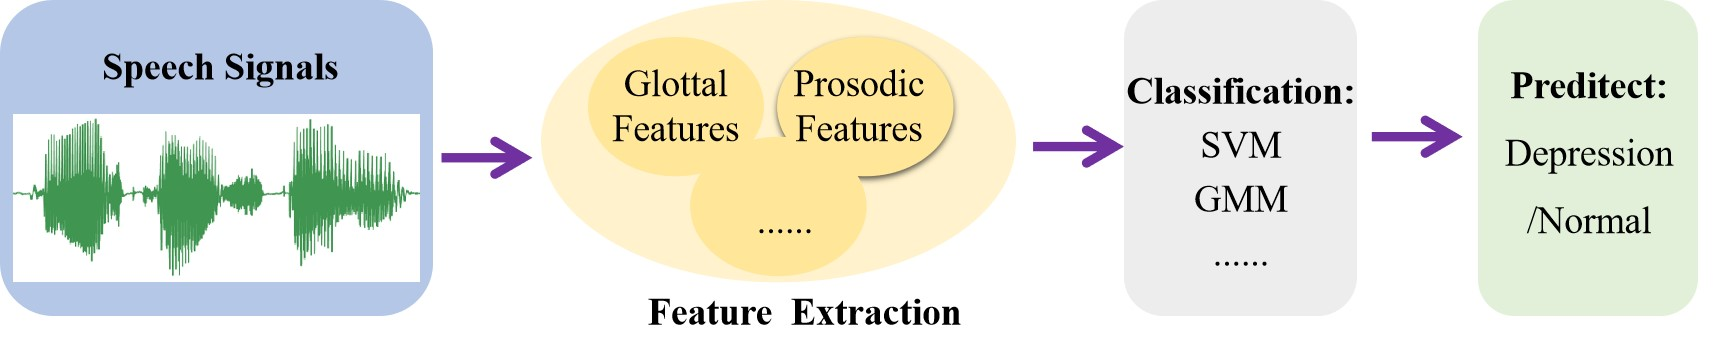
\includegraphics[width=1\linewidth]{Speech_tradition.jpg}
\caption{Flow diagram of speech depression recognition based on traditional machine learning.}
\label{Speech01}
\end{figure}




In the study of speech-based depression recognition, acoustic characteristics principally include prosodic, voice quality, formant, and spectral features\cite{france2000acoustical,moore2003analysis}.
The prosodic features were computed from the speech waveform and included fundamental frequency (F0), log of energy, jitter and shimmer\cite{france2000acoustical}.
Where F0 is one of the most prevalent prosodic features, and its range of variation and decrease in mean value may be related to the severity of depression.
The parameters related to voice quality features are frequency perturbation, amplitude perturbation, and glottal parameters.
The glottal spectrum shows the condition of vocal function, while frequency and amplitude perturbation combined describe the stability of vocal fold vibration\cite{moore2007critical}.
Formant features provide information regarding vocal tract resonance and pronunciation efforts, which represent physical vocal tract properties.
As formant features, the first three formants are commonly employed.
Spectral features are a reflection of the relationship between the shape change of the vocal tract and the articulator movement, and the most widely utilized features are PSD and Mel-scaleFrequency Cepstral Coefficients (MFCC).
The four types of features mentioned above are regularly extracted in frames to generate frame-level Low Level Descriptors (LLDs).
Meanwhile, they can also be extracted directly using feature extraction tools such as OpenSMILE, COVAREP.
A single acoustic feature cannot adequately describe depressive symptoms due to their complexity and variety.
As a result, many researchers have developed and mixed various acoustic features to build higher-performance depression recognition models.
Shankayi et al.\cite{shankayi2012identifying} extracted three categories of features from speech signals: prosodic, vocal tract spectrum, and glottal source. The results showed that using features all together leads to better results than using each category alone.








In traditional speech-based depression recognition studies, SVM\cite{nasir2016multimodal,gong2017topic,cummins2013spectro,helfer2013classification} and Gaussian
Mixture Model (GMM)\cite{helfer2013classification,williamson2013vocal,alghowinem2013comparative} are the two most popularly utilized modeling and classification methods.
Jiang et al.\cite{jiang2017investigation} studied 170 subjects and proposed a computational methodology based on SVM (STEDD). They documented accuracies of 75.96\% for females and 80.30\% for males.
Ooi et al.\cite{ooi2014prediction} studied 30 subjects (15 were at risk of depression and 15 were not at risk) and presented an ensemble method using GMM classifiers that used prosodic and glottal features. They reported a classification result of 74\%.
Alghowinem et al.\cite{alghowinem2013comparative} summarized low-level descriptors and statistical features of 60 subjects (30 controls and 30 depressed patients) and compared four classifiers: GMM, SVM, Hierarchical Fuzzy Signature, and Multilayer Perceptron Neural Network. They concluded that GMM and SVM performed better.






\subsubsection{Speech depression recognition based
on deep learning}


More recently deep learning methods have showed their capacity in many audio based applications. These methods learn discriminative features through multiple layers and performed better than traditional methods.
There are three ways to employ deep learning in this area, depending on the format of the input data.(1)Acoustic features based deep learning model: Traditional acoustic features are put into the deep classifier for training, recognition or prediction;
(2)Spectrogram based deep learning models: Spectrograms are given as input to CNN and low level features are extracted from spectrograms where spectrogram is log scale plot of Short time fourier transform.
(3)End to end deep learning models: Pushing raw signal into deep architecture to let model learn high-level features by itself. Architecture of these models is shown in Fig.\ref{Speech02} .
\begin{figure}
\centering
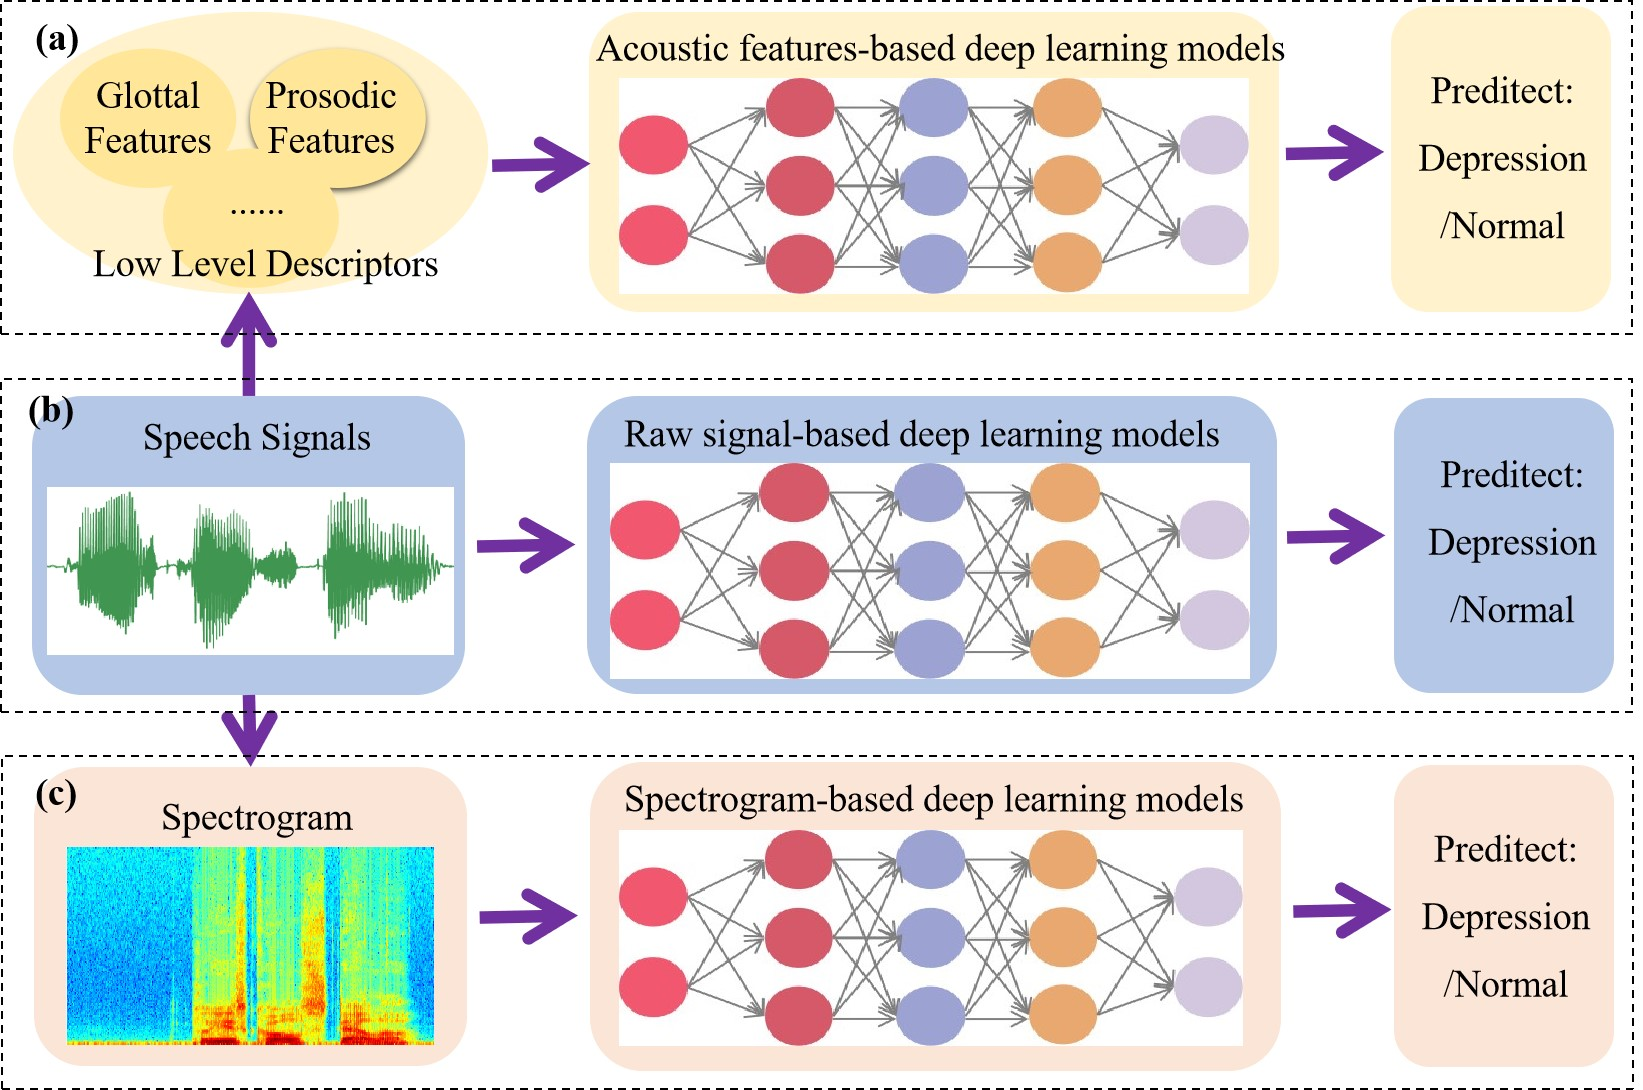
\includegraphics[width=1\linewidth]{Speech_cnn.jpg}
\caption{Flow diagram of speech depression recognition based on deep learning,
with the first to third rows representing acoustic feature-based, spectrogram-based, and end-to-end deep learning models, respectively.
}
\label{Speech02}
\end{figure}

%Figure 2 shows the deep learning based speech depression recognition,


CNN could capture spatial properties of features and has the ability of parallel computing. Therefore, CNN can be used as a classifier for traditional acoustic features.
Well known features, like MFCCs and logMel are fairly simple to extract and have a small number of dimensions which might be more suitable to a low-resource setting than raw signal.
Du et al. \cite{du2018bipolar} presented a novel audio-based approach, called IncepLSTM, which effectively integrated Inception module and LSTM on the 16-dimensional MFCCs to capture multi-scale temporal information for Bipolar Disorder recognition. What's more, experiments were conducted on the AVEC 2018 dataset and the results demonstrated the effectiveness of their proposed approach.



The spectrogram converts the speech signal from a 1-dimensional to a 2-dimensional signal, and it not only represents the dynamic spectral properties of the speech signal but also visualizes the speech.
There are observable differences between the speech spectrograms of depressed and non-depressed people.
In the spectrograms of non-depressed samples, intensity of speech is concentrated more at lower frequencies and low at higher frequencies, whereas, in depressed speech samples, high frequency components also exists with higher intensities and intensity is presented more in short periods of time intervals. Therefore, CNN can use these kind of features from spectrograms to identify depression.
Srimadhur et al.\cite{srimadhur2020end} carried out an investigation on depression detection using spectrogram based CNN. And speech samples from audio visual emotion challenge (AVEC) 2016 DAIC-Woz dataset were utilized for validating the models.
However, most of the input speech features of these studies are based on the amplitude spectrogram, which loses the phase spectrogram information.
Therefore, these speech features may lose some important information related to depression.
In order to make full use of speech information, Fan et al. \cite{fan2022csenet} proposed a complex squeeze-and-excitation network (CSENet) for SDLP, which used the complex spectrogram as the input feature. The complex spectrogram contains all of the speech information both amplitude and phase spectrogram.

%End to end deep learning model: Pushing raw signal into deep architecture to let model learn high-level features by itself.
End to end deep architecture have advantages like that it does not require scholars to have a priori knowledge, deep networks can learn better features and give better classification result. %However, there are a few issues which limit end-to-end deep architectures, such as large-scale
%data supporting, overfitting easily and poor interpretability.
Srimadhur et al.\cite{srimadhur2020end} proposed spectrogram based CNN and end to end CNN models to estimate the severity level of depression on AVEC 2016 DAIC-woz dataset.
Experimental analysis has shown that performance of end to end model is ahead of spectrogram based model and baseline models by an efficiency of 13\%.






\subsubsection{Performance Comparison}
We evaluate the depression recognition method based on speech.
The performance comparisons based
on  traditional machine learning and deep learning are summarized in Table~\ref{tab_1} and Table~\ref{tab_2} respectively.
From the table we obtain the following three observations:

(1)
Comparative analysis of the performances of several classifiers in depression assessment and prediction indicate that the use of an hybrid classifier using GMM and
SVM model gave the best overall classification results\cite{alghowinem2013comparative}. Different fusion methods, namely feature, score and decision fusion
have been also investigated in \cite{alghowinem2013comparative} and it has been demonstrated that : first, amongst the fusion methods, score fusion performed better when combined with
GMM, HFS and MLP classifiers. Second, decision fusion worked best for SVM
(both for raw data and GMM models) and finally, feature fusion exhibited weak
performance compared to other fusion methods.

(2)
Performance of end to end model is better than spectrogram based convolutional neural network model.
Srimadhur\cite{haque2018measuring} conducted an experiment on depression detection using spectrogram based CNN and end to end deep models. Parameter tuning has been performed and comparative analysis has been carried out between two models and best model has been chosen for categorizing the depression state. The results indicated that performance of end to end model was better than the baseline models and spectrogram based convolutional neural network model on DAIC-woz dataset.
Main reason is because of variability in the volume during recording of data samples and normalized the data samples to reduce this affect but there is no changes in the spectrogram of data samples so this spectrogram based convolutional neural networks for depression detection is ineffective to variance of speaker volume.



%%��
%Reason: End to end deep architecture have advantages like that it does not require scholars to have a priori knowledge, deep networks can learn better features and give
%better classification result. However, there are a few issues
%which limit end to end deep architectures, such as large-scale
%data supporting, overfitting easily and poor interpretability.

(3)So far, the most popular method is still the combination of acoustic features and deep classifiers.
As it could solve the problems encountered in hand-crafted features, such as high
threshold, labour cost and low feature utilization rate, deep
learning slowly becomes the leader in the field of machine
learning.
Although the end-to-end model also has better performance, it is difficult to determine the contribution of each module in the architecture due to its end to end characteristics, limiting further performance improvement.
%In a word, end to end deep architectures have not yet been widely used in the field of SDR because of its poor interpretability, flexibility and current limited dataset scale.

%Compared to traditional classifiers, deep classifiers have many advantages, including dealing with complex structures and functions, and unlabelled and incorrectly labelled data.

%In the reported works appreciable performances have been achieved however manual hand-picked features have
%been utilized which requires subject knowledge and used shallow architectures.
%
%End to end deep model is difficult to determine the
%contribution of each module in the architecture due to its end to end characteristics, limiting further performance improvement.


%When used as a classifier, deep classifiers have many advantages, including dealing with complex structures and functions,
%and unlabelled and incorrectly labelled data.
%
%Compared to traditional classifiers, deep classifiers have many advantages, including dealing with complex structures and functions, and unlabelled and incorrectly labelled data.






%When used as a feature extractor,
%deep learning can avoid high labour cost and large-scale loss of feature, and the extensibility is better than traditional method.



% Please add the following required packages to your document preamble:
% \usepackage{booktabs}
\begin{table*}
\caption{ Overview of traditional machine learning based methods for Depression
Assessment from Speech.}
\label{tab_1}
\resizebox{\linewidth}{!}{
\begin{tabular}{@{}ccccc@{}}
\hline
\textbf{Paper} & \textbf{Dataset}     & \textbf{Classifiers}             & \textbf{Metrics} & \textbf{Performance} \\ \hline
Ringeval\cite{ringeval2017avec}       & SEWA                 & Random forest                    & RMSE/MAE         & 7.78/5.72            \\
Low\cite{low2010detection}           & hand-craftes dataset & SVM+GMM                          &                  &                      \\
Alghowinem\cite{alghowinem2013comparative}      & hand-craftes dataset & SVM+GMM+decision fusion          & Accuracy         & 91.67\%              \\
Valster\cite{valstar2013avec}        & AVid-Corpus          & SVR                              & RMSE/MAE         & 14.12/10.35          \\
Cummins\cite{cummins2011investigation} & AVEC2013             & SVM                              & Accuracy         & 82\%                 \\
Meng\cite{meng2013depression}& AVEC2013             & Partial least square regression  & RMSE/MAE         & 11.54/9.78           \\
Williamson\cite{williamson2014vocal} & AVEC2014             & GMM                              & RMSE/MAE         & 8.50/6.52            \\
Nasir\cite{nasir2016multimodal} & DAIC-WOZ             & SVM                              & F1               & 63\%                 \\
Gong\cite{gong2017topic}& DAIC-WOZ             & SVM                              & RMSE/MAE         & 4.99/3.96            \\
Jayawardena\cite{jayawardena2020ordinal}  & DAIC-WOZ             & LR                               & RMSE             & 6.84                 \\
Valstar\cite{valstar2016avec}        & DAIC-WOZ             & SVM + grid search +random forest & RMSE/MAE         & 7.78/5.72            \\ \hline
\end{tabular}}
\end{table*}

\begin{table*}
\caption{Overview of deep learning based methods for depression
assessment from speech.}
\label{tab_2}
\resizebox{\linewidth}{!}{
\begin{tabular}{cccccc}
\hline
\textbf{Paper} & \textbf{Dataset} & \textbf{Features} & \textbf{Classification} & \textbf{Metrics} & \textbf{Performance} \\ \hline
Kang\cite{kang2017deep}& AVEC2014         & LLDs & DNN                     & RMSE/MAE         & 7.37/5.87            \\
Yang\cite{yang2017hybrid}& DAIC-WOZ         & LLDs & DCNN                    & RMSE/MAE         & 5.97/5.16            \\
Al Hannai\cite{al2018detecting}& DAIC-WOZ         & LLDs & LSTM-RNN                & RMSE/MAE         & 10.03/7.60           \\
Dham\cite{dham2017depression}& DAIC-WOZ         & LLDs & FF-NN                   & RMSE/MAE         & 7.63/6.28            \\
Salekin\cite{salekin2018weakly}& DAIC-WOZ         & LLDs & NN2Vec + BLSTMMIL       & F1-score         & 85.44\%              \\
%Alhanai        & DAIC-WOZ         & Raw signal        & LSTM                    & RMSE/MAE         & 6.27/4.97            \\
Zhang\cite{zhang2021depa}& DAIC-WOZ         & Spectrogram       & Transformer             & RMSE/MAE         & 5.73/4.75            \\
Othmani\cite{othmani2021towards}& DAIC-WOZ         & LLDs+ spectrogram & LSTM                    & F1-score         & 82\%                 \\
Srimadhur\cite{haque2018measuring}& DAIC-WOZ         & Raw signal        & CNN                     & F1-score         & 78\%                 \\
Srimadhur\cite{haque2018measuring}& DAIC-WOZ         & Spectrogram       & CNN                     & F1-score         & 66\%                 \\
Ma\cite{ma2016depaudionet}& DAIC-WOZ   & Spectrogram  & Depaudionet      & F1-score  & 52\%                 \\ \hline
\end{tabular}}
\end{table*}







\ifx\allfiles\undefined
% !TEX root = tnnls_relation_gait.tex

% if have a single appendix:
%\appendix[Proof of the Zonklar Equations]
% or
%\appendix  % for no appendix heading
% do not use \section anymore after \appendix, only \section*
% is possibly needed

% use appendices with more than one appendix
% then use \section to start each appendix
% you must declare a \section before using any
% \subsection or using \label (\appendices by itself
% starts a section numbered zero.)
%

%\appendices
%\section{Proof of the First Zonklar Equation}
%Appendix one text goes here.
%
%% you can choose not to have a title for an appendix
%% if you want by leaving the argument blank
%\section{}
%Appendix two text goes here.

% use section* for acknowledgment
% \section*{Acknowledgment}
% The authors would like to thank Prof. Dongbin Zhao for his support to this work.

% Can use something like this to put references on a page
% by themselves when using endfloat and the captionsoff option.
\ifCLASSOPTIONcaptionsoff
  \newpage
\fi

% trigger a \newpage just before the given reference
% number - used to balance the columns on the last page
% adjust value as needed - may need to be readjusted if
% the document is modified later
%\IEEEtriggeratref{8}
% The "triggered" command can be changed if desired:
%\IEEEtriggercmd{\enlargethispage{-5in}}

% references section

% can use a bibliography generated by BibTeX as a .bbl file
% BibTeX documentation can be easily obtained at:
% http://mirror.ctan.org/biblio/bibtex/contrib/doc/
% The IEEEtran BibTeX style support page is at:
% http://www.michaelshell.org/tex/ieeetran/bibtex/
\bibliographystyle{IEEEtran}
% argument is your BibTeX string definitions and bibliography database(s)
\bibliography{IEEEabrv,tnnls_relation_gait}
%
% <OR> manually copy in the resultant .bbl file
% set second argument of \begin to the number of references
% (used to reserve space for the reference number labels box)
%\begin{thebibliography}{1}
%\bibitem{IEEEhowto:kopka}
%H.~Kopka and P.~W. Daly, \emph{A Guide to \LaTeX}, 3rd~ed.\hskip 1em plus
%  0.5em minus 0.4em\relax Harlow, England: Addison-Wesley, 1999.
%\end{thebibliography}

% biography section
%
% If you have an EPS/PDF photo (graphicx package needed) extra braces are
% needed around the contents of the optional argument to biography to prevent
% the LaTeX parser from getting confused when it sees the complicated
% \includegraphics command within an optional argument. (You could create
% your own custom macro containing the \includegraphics command to make things
% simpler here.)
%\begin{IEEEbiography}[{\includegraphics[width=1in,height=1.25in,clip,keepaspectratio]{mshell}}]{Michael Shell}
% or if you just want to reserve a space for a photo:

%\begin{IEEEbiography}{Michael Shell}
%Biography text here.
%\end{IEEEbiography}
%
%% if you will not have a photo at all:
%\begin{IEEEbiographynophoto}{John Doe}
%Biography text here.
%\end{IEEEbiographynophoto}

% insert where needed to balance the two columns on the last page with
% biographies
% \newpage

%\begin{IEEEbiographynophoto}{Jane Doe}
%Biography text here.
%\end{IEEEbiographynophoto}

%\begin{IEEEbiography}[{\includegraphics[width=1in,height=1.25in,clip,keepaspectratio]{photos/hsh.pdf}}]{Saihui Hou}
%% \begin{IEEEbiographynophoto}{Saihui Hou}
%	received the B.E. and Ph.D. degrees from University of Science and Technology of China in 2014 and 2019, respectively.
%    %
%    He is currently an Assistant Professor with School of Artificial Intelligence, Beijing Normal University.
%    %
%    His research interests include computer vision and machine learning.
%    %
%    He focuses on gait recognition which aims to identify different people according to the walking patterns.
%% \end{IEEEbiographynophoto}
%\end{IEEEbiography}
%
%\begin{IEEEbiography}[{\includegraphics[width=1in,height=1.25in,clip,keepaspectratio]{photos/lx.pdf}}]{Xu Liu}
%% \begin{IEEEbiographynophoto}{Xu Liu}
%	received the B.E. and Ph.D. degrees from University of Science and Technology of China in 2013 and 2018, respectively.
%    %
%    He is currently a Research Scientist with Watrix Technology Limited Co. Ltd.
%    %
%    His research interests include gait recognition, object detection and image segmentation.
%% \end{IEEEbiographynophoto}
%\end{IEEEbiography}
%
%\begin{IEEEbiography}[{\includegraphics[width=1in,height=1.25in,clip,keepaspectratio]{photos/ccs.pdf}}]{Chunshui Cao}
%% \begin{IEEEbiographynophoto}{Chunshui Cao}
%	received the B.E. and Ph.D. degrees from University of Science and Technology of China in 2013 and 2018, respectively.
%    %
%    During his Ph.D. study, he joined Center for Research on Intelligent Perception and Computing, National Laboratory of Pattern Recognition, Institute of Automation, Chinese Academy of Sciences.
%    %
%    From 2018 to 2020, he worked as a Postdoctoral Fellow with PBC School of Finance, Tsinghua University.
%    %
%    He is currently a Research Scientist with Watrix Technology Limited Co. Ltd.
%    %
%    His research interests include pattern recognition, computer vision and machine learning.
%% \end{IEEEbiographynophoto}
%\end{IEEEbiography}
%
%\begin{IEEEbiography}[{\includegraphics[width=1in,height=1.25in,clip,keepaspectratio]{photos/hyz.pdf}}]{Yongzhen Huang}
%% \begin{IEEEbiographynophoto}{Yongzhen Huang}
%	received the B.E. degree from Huazhong University of Science and Technology in 2006, and the Ph.D. degree from Institute of Automation, Chinese Academy of Sciences in 2011.
%    %
%    He is currently an Associate Professor with School of Artificial Intelligence, Beijing Normal University.
%    %
%    He has published one book and more than 80 papers at international journals and conferences such as TPAMI, IJCV, TIP, TSMCB, TMM, TCSVT, CVPR, ICCV, ECCV, NIPS, AAAI.
%    %
%    His research interests include pattern recognition, computer vision and machine learning.
%% \end{IEEEbiographynophoto}
%\end{IEEEbiography}


\end{document}

\fi
